\section{Introduction}

Advanced analytics involves a range of sophisticated data analysis methods that are crucial in the business context. 
These techniques span a broad spectrum of complexity and value, encompassing four primary categories: descriptive, diagnostic, predictive, and prescriptive analytics.
The ultimate aim is to uncover hidden patterns, predict future trends, and make data-driven decisions.
The four categories of analysis are as follows:
\begin{enumerate}
    \item \textit{Descriptive}: this type of analysis focuses on examining historical data to identify patterns and trends.
        It provides a foundational understanding of past business performance.
    \item \textit{Diagnostic}: diagnostic analytics seeks to understand the causes behind specific events. 
        It uncovers relationships and correlations within the data, helping to identify why things occurred.
    \item \textit{Predictive}: predictive analytics uses historical data to forecast potential future outcomes. 
        By analyzing past trends, it provides probabilities for future events, helping businesses anticipate what might happen next.
    \item \textit{Prescriptive}: this form of analysis goes a step further by recommending specific actions to influence future outcomes. 
        It suggests strategies to help achieve desired goals, guiding decision-making processes.
\end{enumerate}
\noindent Data refers to raw, unprocessed facts (the basic unit of measurable information). 
While it can be stored and transmitted, it's not immediately useful until it's processed and analyzed.
In contrast, information is data that has been processed and organized, making it meaningful and useful. 
Information provides insights into what is being measured and observed, helping to understand the underlying patterns.

In business, data must be transformed into valuable insights through processing and analysis. 
This transformation allows organizations to make informed decisions, guiding them toward their goals.

Additionally, knowledge arises when information is combined with experience, expertise, and authoritative judgment, leading to actionable decisions.

The following diagram illustrates the different levels of data analytics and their application in decision-making.
\begin{figure}[H]
    \centering
    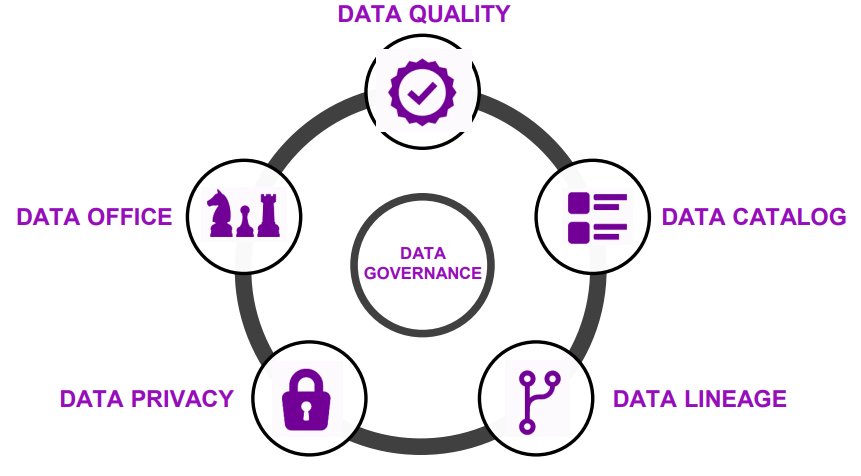
\includegraphics[width=0.5\linewidth]{images/bis5.png}
    \caption{Data analytics levels}
\end{figure}

\subsection{SGD approach}
Business agility refers to an organization's ability to rapidly adapt to market changes, both internally and externally. 
Achieving true business agility is only possible if an organization becomes deeply data-driven. 
SDG Group helps businesses achieve this by co-creating tailored solutions with customers, leveraging data and analytics services. 
This is accomplished through a unique blend of business domain expertise, cutting-edge technologies, and industry-leading talent.

As pioneers in AI, Data, and Analytics consulting, SDG Group is committed to unlocking the hidden potential of organizations. 
We achieve this by offering in-depth analytics expertise that empowers businesses to thrive in a fast-changing world.

SDG Group's approach is built on three core pillars of Triple Expertise, combining business process knowledge, technological prowess, and partnerships with leading software providers.
This enables us to deliver innovative, state-of-the-art solutions and advanced analytics capabilities. Our pillars are:
\begin{itemize}
    \item Practice expertise.
    \item Business insights.
    \item Technological knowledge.
\end{itemize}
\noindent At SDG Group, career development begins with a shared foundation and evolves based on individual specialization. 
Professionals have the opportunity to advance along a career path that leads to key positions such as Executive Manager or Subject Matter Expert, depending on their level of expertise and focus area.

\subsection{Business intelligence}
Business Intelligence (BI) primarily focuses on historical reporting, utilizing descriptive and diagnostic analytics to help organizations understand past performance. 
By leveraging this information, businesses can gain competitive advantages, make informed decisions, and achieve long-term stability. 
Advanced analytics, which includes predictive and prescriptive capabilities, builds upon this foundation, enabling even deeper insights into future trends and optimal actions.

A central aspect of BI is the ability to collect data and respond based on the insights derived. 
It involves understanding the interrelationships among various pieces of data and using that understanding to guide actions towards achieving desired outcomes. 
BI systems use fact-based support to enhance business decision-making.

\begin{definition}[\textit{Business intelligence}]
    Business Intelligence is a set of methodologies, processes, architectures, and technologies that transform raw data into meaningful and actionable information, enabling more effective strategic, tactical, and operational decision-making.
\end{definition}
\noindent A BI system is typically designed through the following steps:
\begin{enumerate}
    \item \textit{Data identification and structuring}: identifying relevant data and organizing it in a usable format.
    \item \textit{Expected output definition}: defining the expected results and objectives of the analysis.
    \item \textit{Database model and design}: creating the appropriate data structures to store and manage the data.
    \item \textit{Dashboards and visual design}: developing user-friendly dashboards and visualizations to present the data in a meaningful way.
\end{enumerate}
\noindent The following diagram shows the typical architecture of a Business Intelligence system.
\begin{figure}[H]
    \centering
    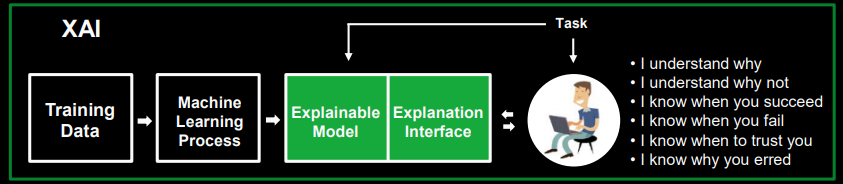
\includegraphics[width=0.5\linewidth]{images/bis6.png}
    \caption{Standard architecture}
\end{figure}
There are three primary levels of BI systems, catering to different types of users:
\begin{enumerate}
    \item \textit{Technical BI} (IT end users): focused on the infrastructure and backend of BI systems.
    \item \textit{Self-service BI} (aalysts): allowing business analysts to explore data and generate insights independently.
    \item \textit{End-user BI} (everyone): designed for general users across the organization to access insights and make data-driven decisions.
\end{enumerate}

In today's data-driven landscape, transforming raw data into actionable knowledge and tangible value is essential for success. 
The following considerations are critical:
\begin{enumerate}
    \item \textit{Quality data}: start with accurate and reliable data.
    \item \textit{Context matters}: understand the context in which the data operates to ensure meaningful analysis.
    \item \textit{Business relevance}: focus on data that directly impacts business goals and objectives.
    \item \textit{Agility}: be prepared to adapt quickly as the data landscape evolves.
\end{enumerate}

The diagram below illustrates the lifecycle of business information, from raw data to valuable insights.

\begin{figure}[H]
    \centering
    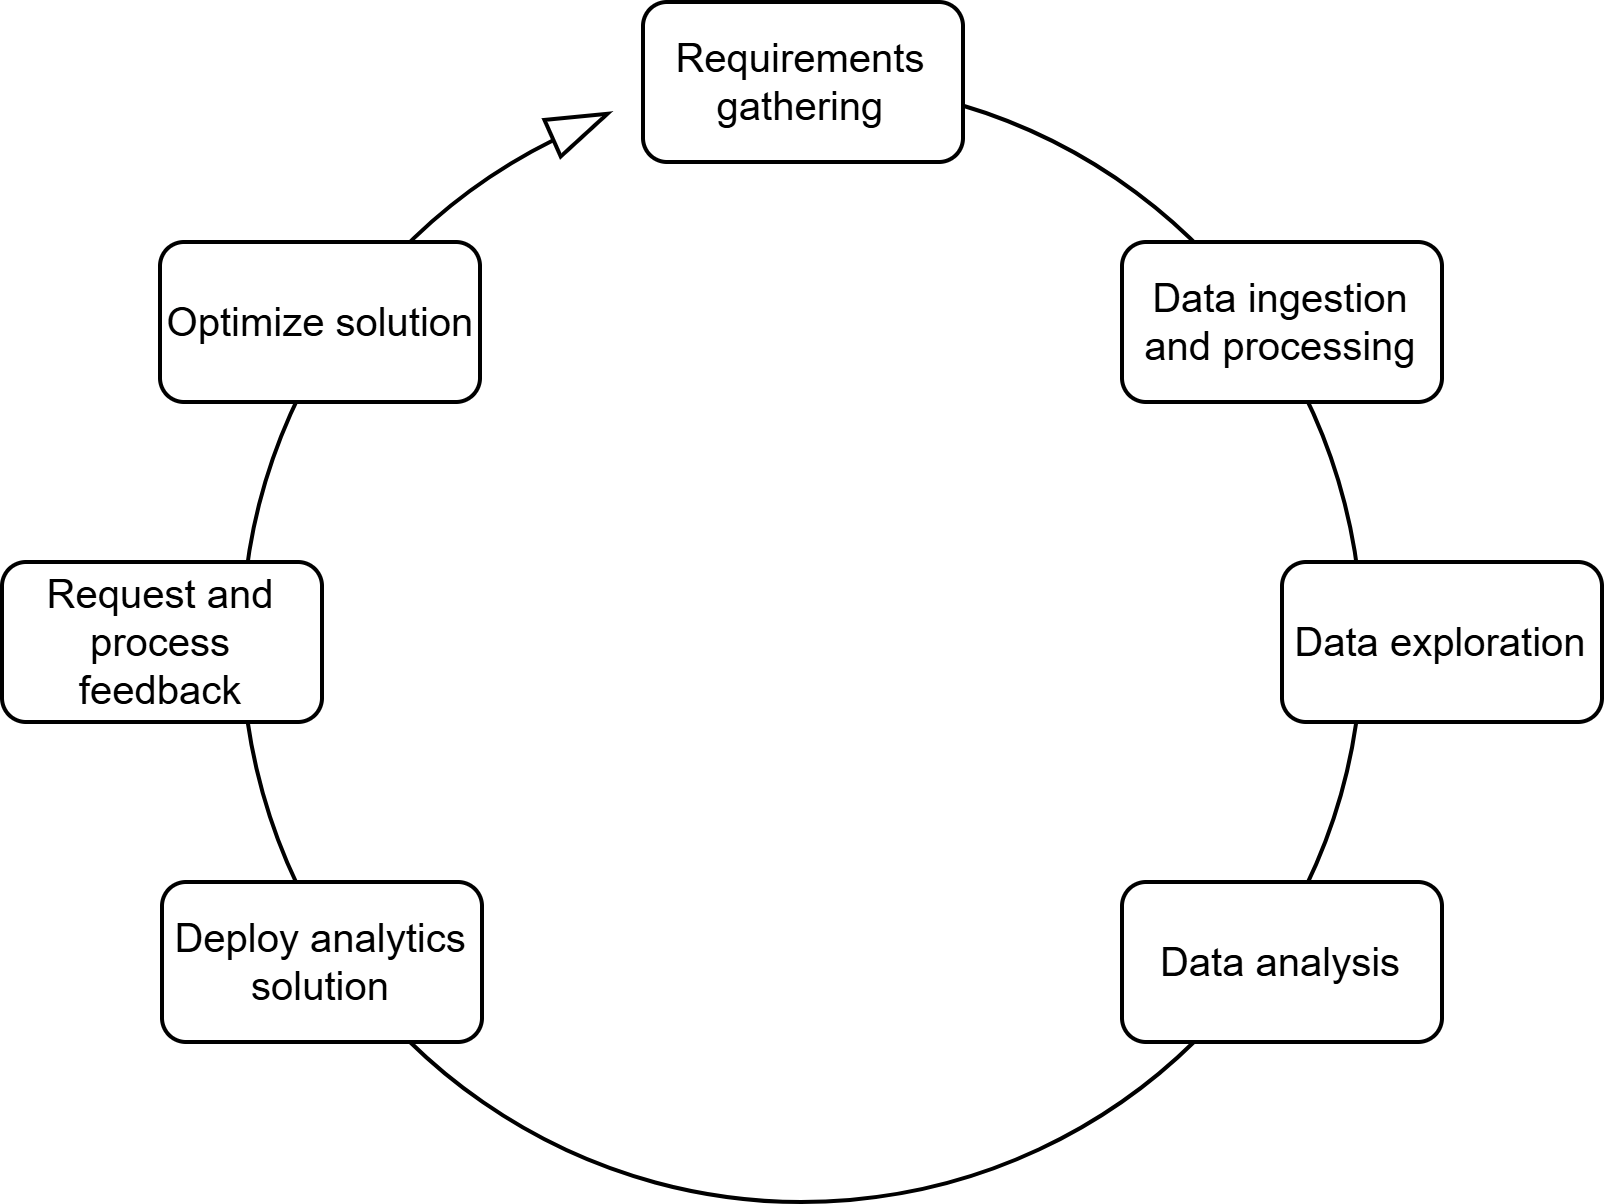
\includegraphics[width=0.5\linewidth]{images/bis7.png}
    \caption{Business information lifecycle}
\end{figure}